\documentclass[]{DINOReportMemo}
\usepackage{DINO_C-REx}
\usepackage{colortbl}


\newcommand{\ModuleName}{Image Generation} %edit this!
\newcommand{\subject}{Systems Engineering Report: Magnitude to Stellar Flux Conversion} %edit this!
\newcommand{\status}{Initial Version}
\newcommand{\preparer}{Matt Muszynski} %edit this!
\newcommand{\summary}{Description, analysis, and recommendation for converting the stellar magnitudes presented in the Tycho-2 catalog to blackbody curves for each star modeled.} %edit this
\usepackage{float}
\usepackage{rotating}
\usepackage{pdflscape}

\begin{document}

\makeCover
%
% enter the revision documentation here
% to add more lines, copy the table entry and the \hline, and paste after the current entry.
%
\pagestyle{empty}
{\renewcommand{\arraystretch}{2}
\noindent
\begin{longtable}{|p{0.5in}|p{4.5in}|p{1.14in}|}
\hline
{\bfseries Rev}: & {\bfseries Change Description} & {\bfseries By} \\
\hline
1.0 & Initial Release & Matt Muszynski \\ %edit this
1.1 & Revised Fig \ref{T_scatter} and eqn \ref{empirical_T_func} after finding an error in code. Removed Johnson Magnitude Plots/Equations. Added analysis of Calculated Tycho Magnitudes & Matt Muszynski \\
\hline

\end{longtable}
}

\newpage
\setcounter{page}{1}
\pagestyle{fancy}

\tableofcontents
~\\ \hrule ~\\

\newpage
\section{Overview}\\\\
Because the DINO C-REx Camera Team has been unable to find a reasonably simple method for converting stellar magnitudes (especially Tycho magnitudes) to stellar blackbody spectra, we have attempted to derive our own model that is presented here. The model gives a surprising level of accuracy given its somewhat crude approximations, and given the number of stars modeled in DINO C-REx, we believe that it is the best way to produce wavelength dependent spectra for all stars given the data from the Tycho-2 catalog. This document describes the assumptions, method, and results of the DINO C-REx conversion model and is presented for feedback and/or approval from Aerospace Corporation.

\section{Method} \\

The DINO C-REx stellar spectrum model begins by deriving a theoretical relationship for Johnson color index $(B-V)_J$ and Temperature $T$ as well as between Tycho color index $(B-V)_T$ and $T$ for blackbodies using Vega as a zero point for each filter. We then use this relationship to find blackbody curves for each star, and use the visual magnitude of each to calcualte a reduction term that accounts for the size of the star and its distance from the solar system. 

\section{Assumptions}
\begin{enumerate}
    \item All stars in the DINO C-REx model are perfect blackbodies.
    \item All points within the solar system are equidistant from any star (other than the sun).
\end{enumerate}
\section{Color Index and Temperature Correlation} \\\\
The first goal of the model is to derive a relationship between the temperature of a star and its color index. This begins by calculating the flux of a generic star and a reference star (here we use Vega) in both the $B$ and $V$ bands as measured from a point in the solar system:
\begin{equation} \label{flux_eqns}
\begin{split}
    F_{B,*} &= \frac{4\pi^2r_*^2}{4\pi d_*^2} \int_0^\infty  B_{\lambda}(\lambda,T)S_{B,\lambda}(\lambda)d\lambda \\
    F_{V,*} &= \frac{4\pi^2r_*^2}{4\pi d_*^2} \int_0^\infty  B_{\lambda}(\lambda,T)S_{V,\lambda}(\lambda)d\lambda \\
    F_{B,Vega} &= \frac{4\pi^2r_{Vega}^2}{4\pi d_{Vega}^2} \int_0^\infty  B_{\lambda}(\lambda,T)S_{B,\lambda}(\lambda)d\lambda \\
    F_{V,Vega} &= \frac{4\pi^2r_{Vega}^2}{4\pi d_{Vega}^2} \int_0^\infty  B_{\lambda}(\lambda,T)S_{V,\lambda}(\lambda)d\lambda
\end{split}
\end{equation}
Where  $B_{\lambda}(\lambda,T)$ is the Planck function:
\begin{equation}
    B_{\lambda}(\lambda,T) = \frac{2hc^2}{\lambda^5}\frac{1}{e^{\frac{hc}{\lambda k_B T}}-1}
\end{equation}
$S_{\lambda}(\lambda)$ is the sensitivity of the filter of interest\footnote{As given numerically by https://arxiv.org/pdf/1412.1474.pdf}, $h$ is the Planck constant, $c$ is the speed of light, and $k_B$ is the Boltzmann constant. The $\frac{4\pi^2r_*^2}{4\pi d_*^2}$ at the front of each expression accounts for the size of the star, its distance from the solar system, and the inverse steradian term present in $\int_0^\infty  B_{\lambda}(\lambda,T) d\lambda$.

\begin{figure*}[t!]
    \centering
    \begin{subfigure}
        \centering
        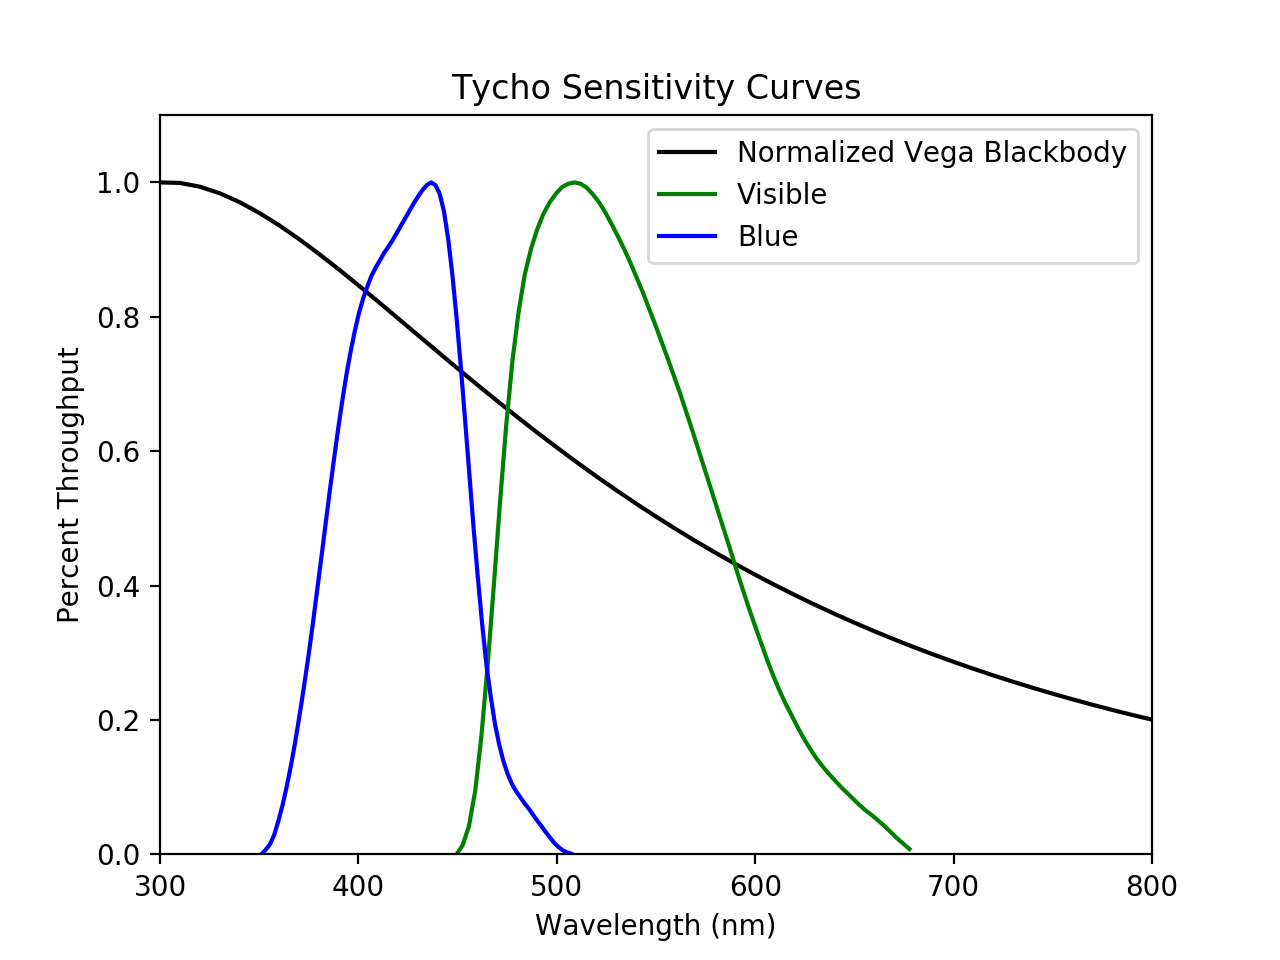
\includegraphics[height=2.3in]{tycho_curves}
    \end{subfigure}%
    ~ 
    \begin{subfigure}
        \centering
        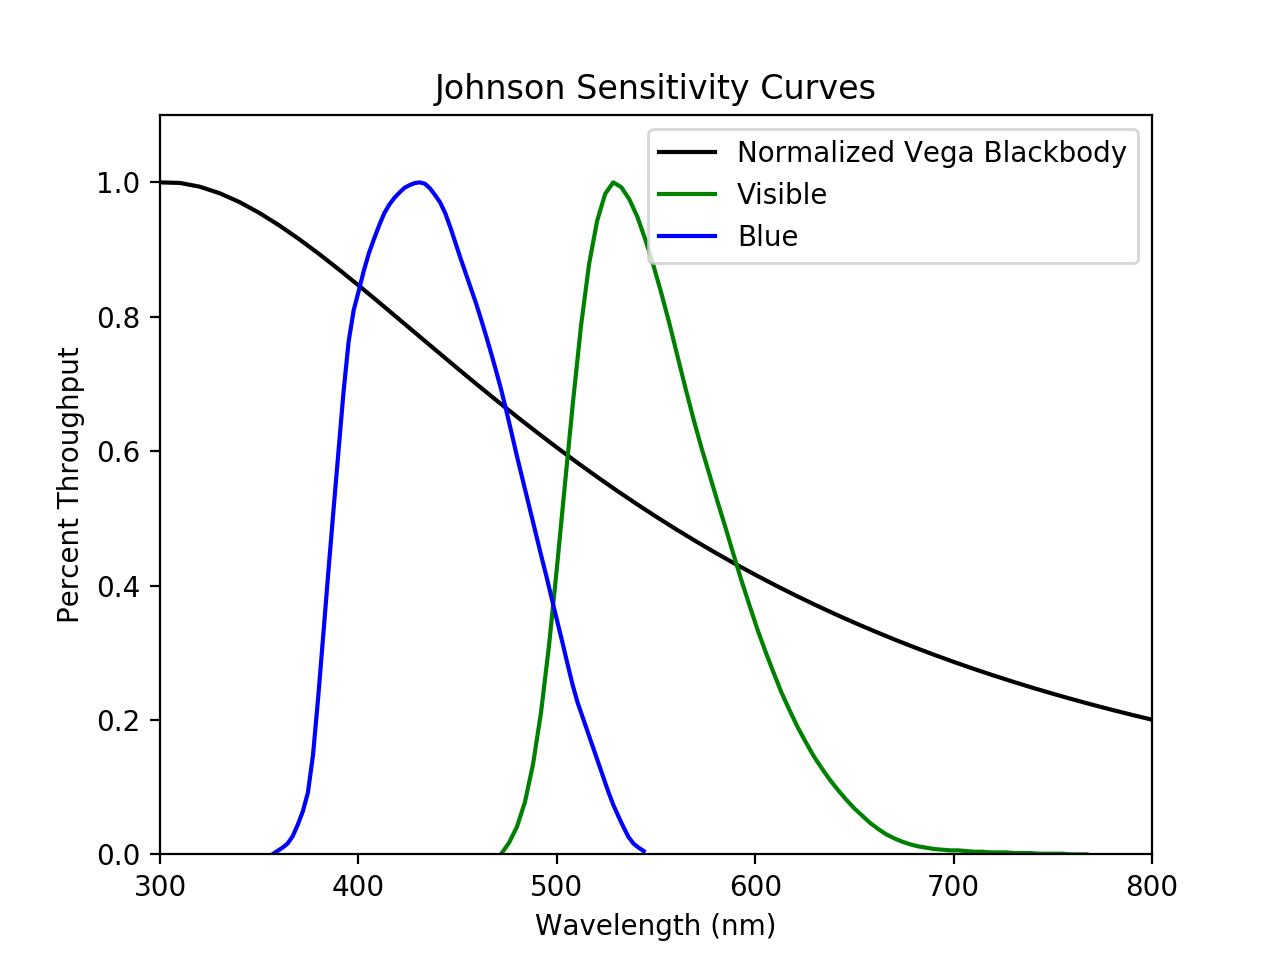
\includegraphics[height=2.3in]{johnson_curves}
    \end{subfigure}
    \caption{Sensitivity curves for B and V filters for both Tycho and Johnson. Both are overlaid with a normalized blackbody for Vega with an effective temperature of 9550K.}
\end{figure*}


Given these fluxes, we find the magnitude of our generic star in each band:
\begin{equation}
\begin{split}
    B_* &= -2.5\log_{10}\left(\frac{F_{B,*}}{F_{B,Vega}}\right) \\
    V_* &= -2.5\log_{10}\left(\frac{F_{V,*}}{F_{V,Vega}}\right)
\end{split}
\end{equation}
Further, we can solve for the color index of the star as only a function of its temperature:
\begin{equation}
\begin{split}
    (B-V)_* &= -2.5\log_{10}\left(\frac{F_{B,*}}{F_{B,Vega}}\right) +2.5\log_{10}\left(\frac{F_{V,*}}{F_{V,Vega}}\right) \\
    (B-V)_* &= -2.5\log_{10}\left(\frac{F_{B,*}}{F_{B,Vega}}\frac{F_{V,Vega}}{F_{V,*}}\right)
\end{split}
\end{equation}

Substituting the flux expressions from equation \ref{flux_eqns}, we find that all terms outside of the integrals cancel, meaning that we don't have to account for the size or distance of either our generic star or of Vega:
\begin{equation}\label{BV_T_rel}
\begin{split} 
    (B-V)_* &= -2.5\log_{10}\left(\frac{
    \int_0^\infty  B_{\lambda}(\lambda,T_*)S_{B,\lambda}(\lambda)d\lambda
    \int_0^\infty  B_{\lambda}(\lambda,T_{Vega})S_{V,\lambda}(\lambda)d\lambda
    }{
    \int_0^\infty  B_{\lambda}(\lambda,T_*)S_{V,\lambda}(\lambda)d\lambda
    \int_0^\infty  B_{\lambda}(\lambda,T_{Vega})S_{B,\lambda}(\lambda)d\lambda
    }
    \right)
\end{split}
\end{equation}
Solving this expression computationally for many $T_*$'s allows us to create a plot of color index versus Temperature (fig \ref{theory_curve}):

\begin{figure}[h]
\centering
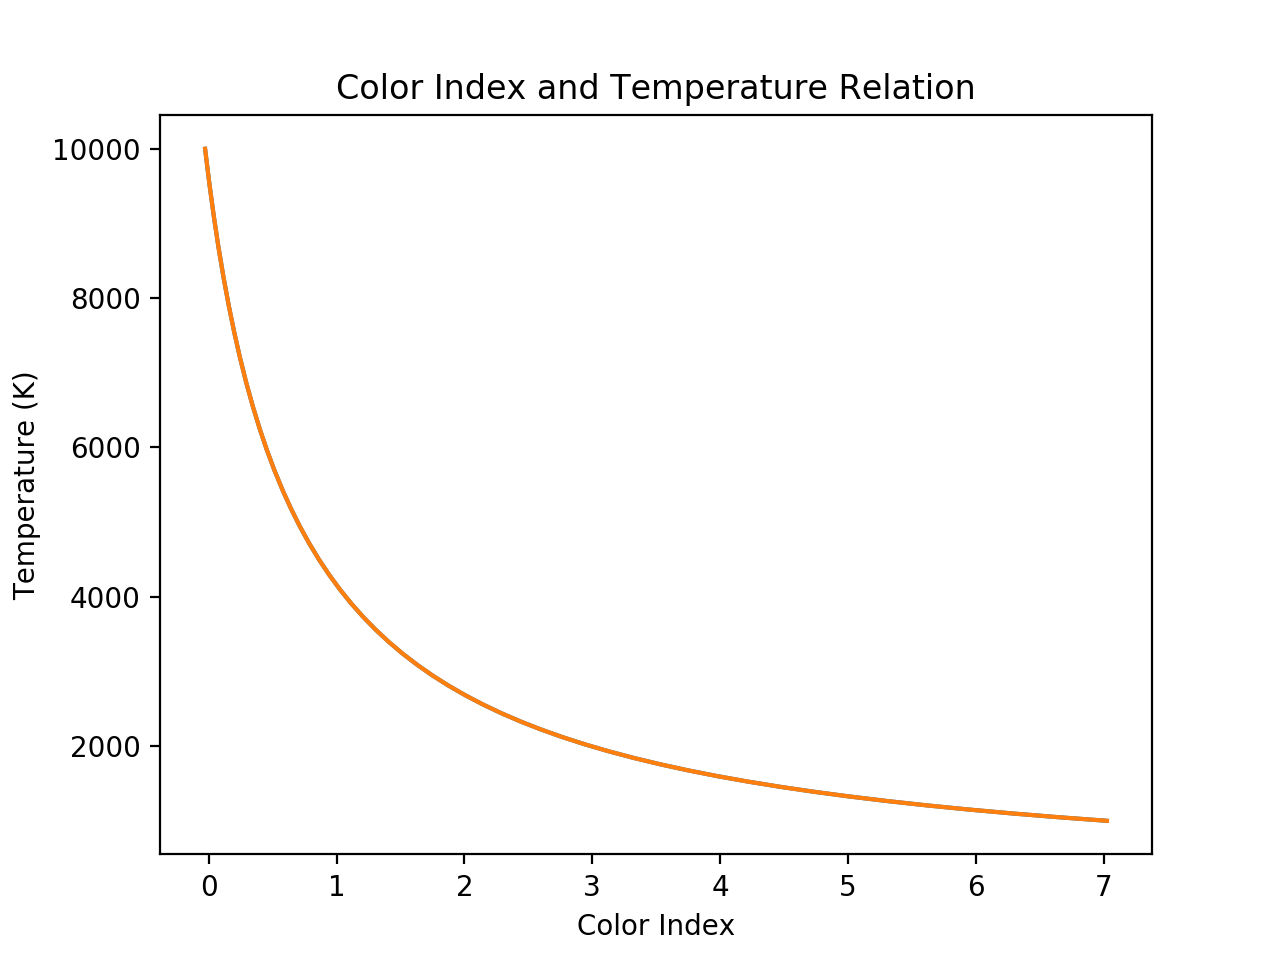
\includegraphics[height=3in]{BV_vs_T}
\caption{Color index versus temperature for Tycho magnitude system.}
\label{theory_curve}
\end{figure}
From this model, we use the Python package lmfit to perform a non-linear least squares fit for each curve using the Levenberg-Marquardt algorithm.\footnote{https://en.wikipedia.org/wiki/Levenberg-Marquardt\_algorithm} This provides the following relationship:


\begin{equation}\label{empirical_T_func}
    T = 6765.93040\Big[0.93431989+(B-V)_T\Big]^{-0.68853863}
\end{equation}
\begin{figure*}[t!]
    \centering
    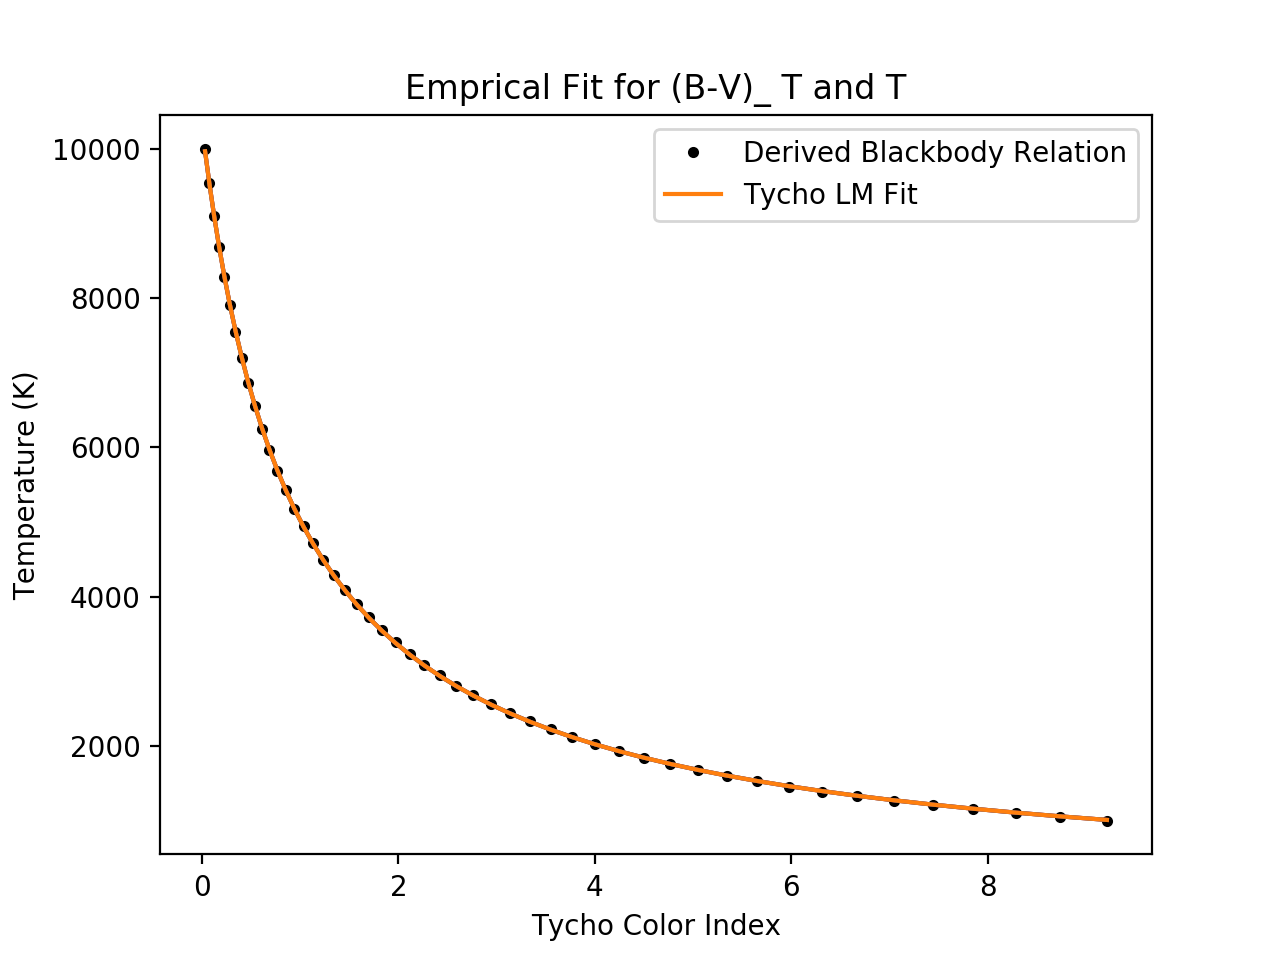
\includegraphics[height=3in]{tycho_lm_fit}
    \caption{Results of the Levenberg-Marquardt fits on Color Index/Temperature relation stated in Eqn. \ref{BV_T_rel}}
\end{figure*}

The DINO C-REx Camera Team has verified this model by looking up the published temperatures of well-known bright stars. Plotting computed temperature versus published temperature produces figure \ref{T_scatter}. Zooming in to the domain between 2500K and 12500K shows a reasonably high fidelity fit for the vast majority of stars. Because the model treats all stars the same, we expect the model to perform similarly for all stars main sequence or otherwise. Mitigation for both the $>$12500K tail of the distribution and the extreme outlier Gamma Velorum are presented below in the sections titled  \textbf{Recommendations} and \textbf{Caveats} respectively.

\begin{figure*}[t!]
    \centering
    \begin{subfigure}
        \centering
        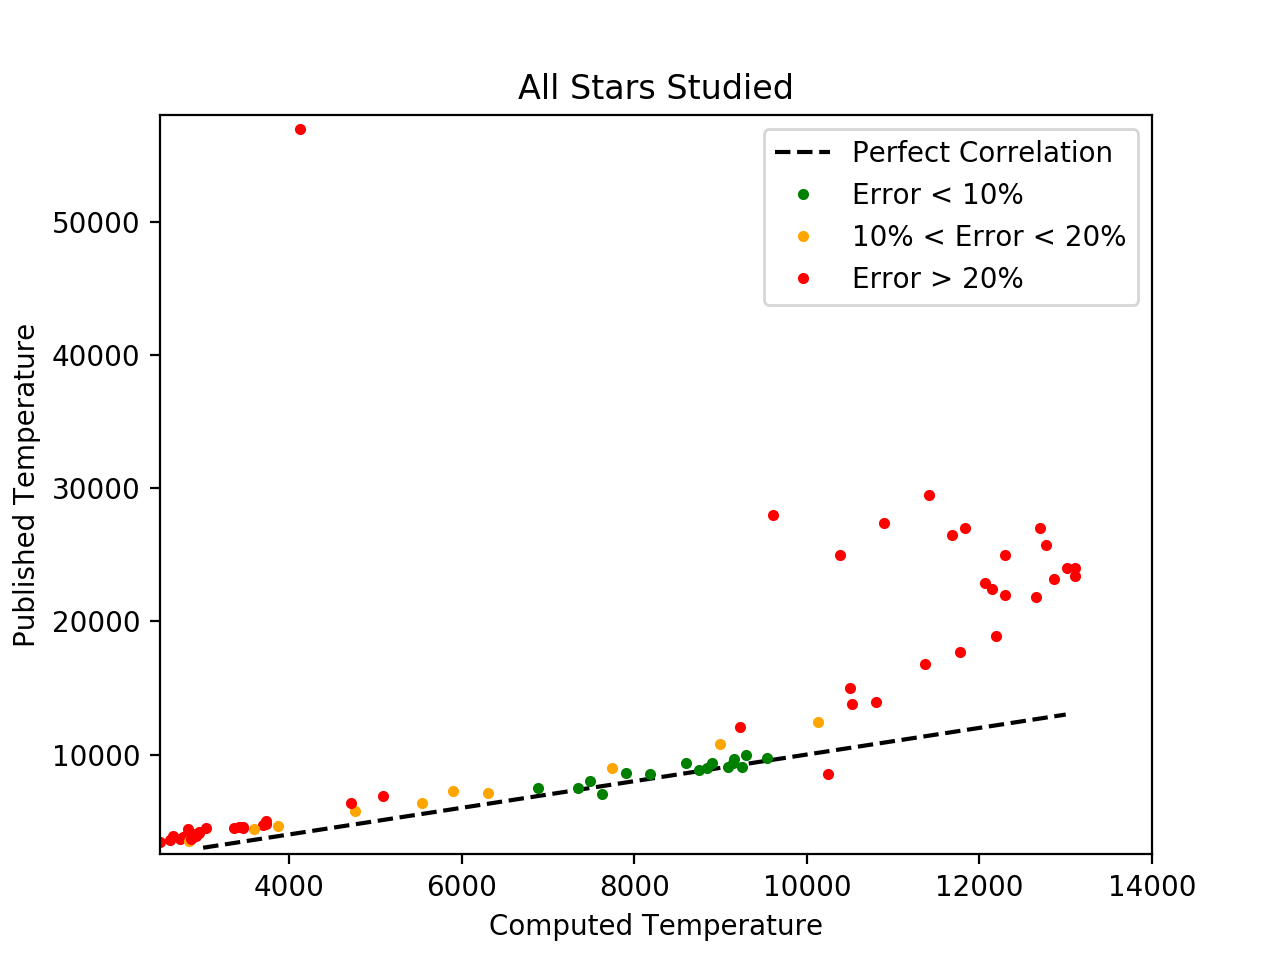
\includegraphics[height=2.3in]{all_stars_scatter}
    \end{subfigure}%
    ~ 
    \begin{subfigure}
        \centering
        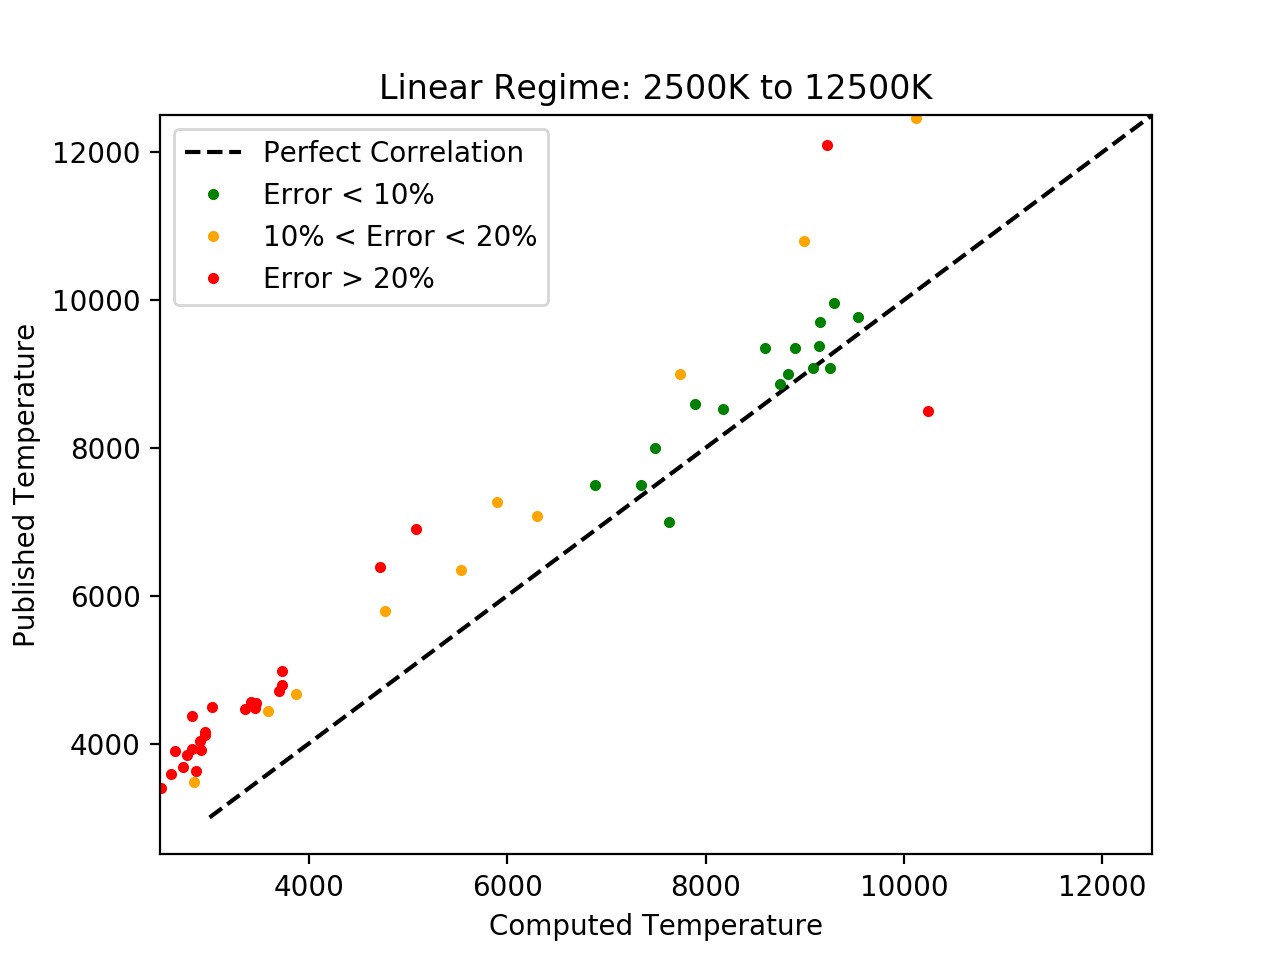
\includegraphics[height=2.3in]{linear_regime_scatter}
    \end{subfigure}
    \caption{Illustration of the success (and failure) of the method for 76 of the brightest stars showing a roughly linear relationship for stars between 2500K and 12500K and a high divergence elsewhere. See recommendations below for how to deal with divergence.}
    \label{T_scatter}
\end{figure*}



\section{Computing Incident  Intensity from Color Index and Relative Visual Magnitude.} \\
Given this model for temperature, the full-specturum blackbody flux is easily calculated via the equation:

\begin{equation}\label{full_flux_expression}
    F(\lambda,T) = \pi\frac{r^2_*}{d^2_*}B_\lambda(\lambda,T)
\end{equation}

However, as we do not have reliable values for $r_*$ or $d_*$ for the vast majority of stars in the Tycho catalog, we must approximate the ratio of their squares. To achieve this, we return to the equation:

\begin{equation}
\begin{split}
V_* &= -2.5\log_{10}\left(\frac{F_{V,*}}{F_{V,Vega}}\right) \\
V_* &= -2.5\log_{10}\left(\frac{
\frac{4\pi^2r_*^2}{4\pi d_*^2} \int_0^\infty  B_{\lambda}(\lambda,T_*)S_{V,\lambda}(\lambda)d\lambda
}{\frac{4\pi^2r_{Vega}^2}{4\pi d_{Vega}^2} \int_0^\infty  B_{\lambda}(\lambda,T_{Vega})S_{V,\lambda}(\lambda)d\lambda}\right) \\
10^{-\frac{V_*}{2.5}} &= \frac{
\frac{r_*^2}{d_*^2} \int_0^\infty  B_{\lambda}(\lambda,T_*)S_{V,\lambda}(\lambda)d\lambda
}{\frac{r_{Vega}^2}{d_{Vega}^2} \int_0^\infty  B_{\lambda}(\lambda,T_{Vega})S_{V,\lambda}(\lambda)d\lambda} 
\end{split}
\end{equation}
\begin{equation} \label{ratio_of_squares}
\frac{r_*^2}{d_*^2} =
10^{-\frac{V_*}{2.5}}
\frac{r^2_{Vega}}{d^2_{Vega}}
\frac{\int_0^\infty  B_{\lambda}(\lambda,T_{Vega})S_{V,\lambda}(\lambda)d\lambda}{\int_0^\infty  B_{\lambda}(\lambda,T_*)S_{V,\lambda}(\lambda)d\lambda}
\end{equation}

Combining equations \ref{full_flux_expression} and \ref{ratio_of_squares}, we have a full expression for the flux of any star reaching the camera. Importantly here, the distance and radius of Vega do not cancel. DINO C-REx uses the following constants for $T_{Vega}$
\footnote{Kinman, T.; et al. (2002), "The determination of Teff for metal-poor A-type stars using V and 2MASS J, H and K magnitudes", Astronomy and Astrophysics, 391 (3): 1039-1052}, $r_{Vega}$
\footnote{Derived from Yoon, Jinmi; et al. (January 2010), "A New View of Vega's Composition, Mass, and Age", The Astrophysical Journal, 708 (1): 71-79. Original source gives an equatorial radius of $2.818 R_\astrosun$ and a polar radius of $2.362 R_\astrosun$. The value of $2.6496 R_{\astrosun}$ stated above is for a spherical star with the same surface area.}, and $d_{Vega}$
\footnote{Derived from The Hipparcos Catalogue -- RA: 14h-19h, HIP: 68301-93276, https://www.cosmos.esa.int/documents/532822/552851/vol9_all.pdf/50682119-3f37-4048-8f3a-e10961614b44}:
\begin{equation}
\begin{split}
    T_{Vega} &= 9,602 K  \\
    r_{Vega} &= 2.6496 R_{\astrosun} \\
    d_{Vega} &= 25.04 ly \\
\end{split}
\end{equation}

Using this relationship, we use the computed temperatures to compute blackbody curves and the received flux for each star.
\begin{equation}
\begin{split}
    F_{B,*} &= \frac{4\pi^2r_*^2}{4\pi d_*^2}\int_0^\infty B_\lambda(\lambda,T_*)S_B(\lambda)d\lambda \\
    F_{V,*} &= \frac{4\pi^2r_*^2}{4\pi d_*^2}\int_0^\infty V_\lambda(\lambda,T_*)S_C(\lambda)d\lambda \\
\end{split}
\end{equation}

And the Tycho B and V magntiudes of each star:

\begin{equation}
\begin{split}
   B_{T,*} &= -2.5\log_{10}\left(\frac{F_{B,*}}{F_{B,Vega}}\right) \\
   V_{T,*} &= -2.5\log_{10}\left(\frac{F_{V,*}}{F_{V,Vega}}\right) \\
\end{split}
\end{equation}

Computing $V_T$ $B_T$ shows a good fit with the data published in the Tycho catalog, especially for $V_T$ (as should be expected as $V_T$ was used directly to compute $\frac{r_*^2}{d_*^2}$. The error between published and calculated $V_T$ has a mean of $-5.646e-10$ and a standard deviation of $1.414e-16$, both consistent with machine error. The error between published and calculated $B_T$ has a mean of $-2.221e-3$ and a standard deviation of $2.973e-3$.

\begin{figure*}[t!]
    \centering
    \begin{subfigure}
        \centering
        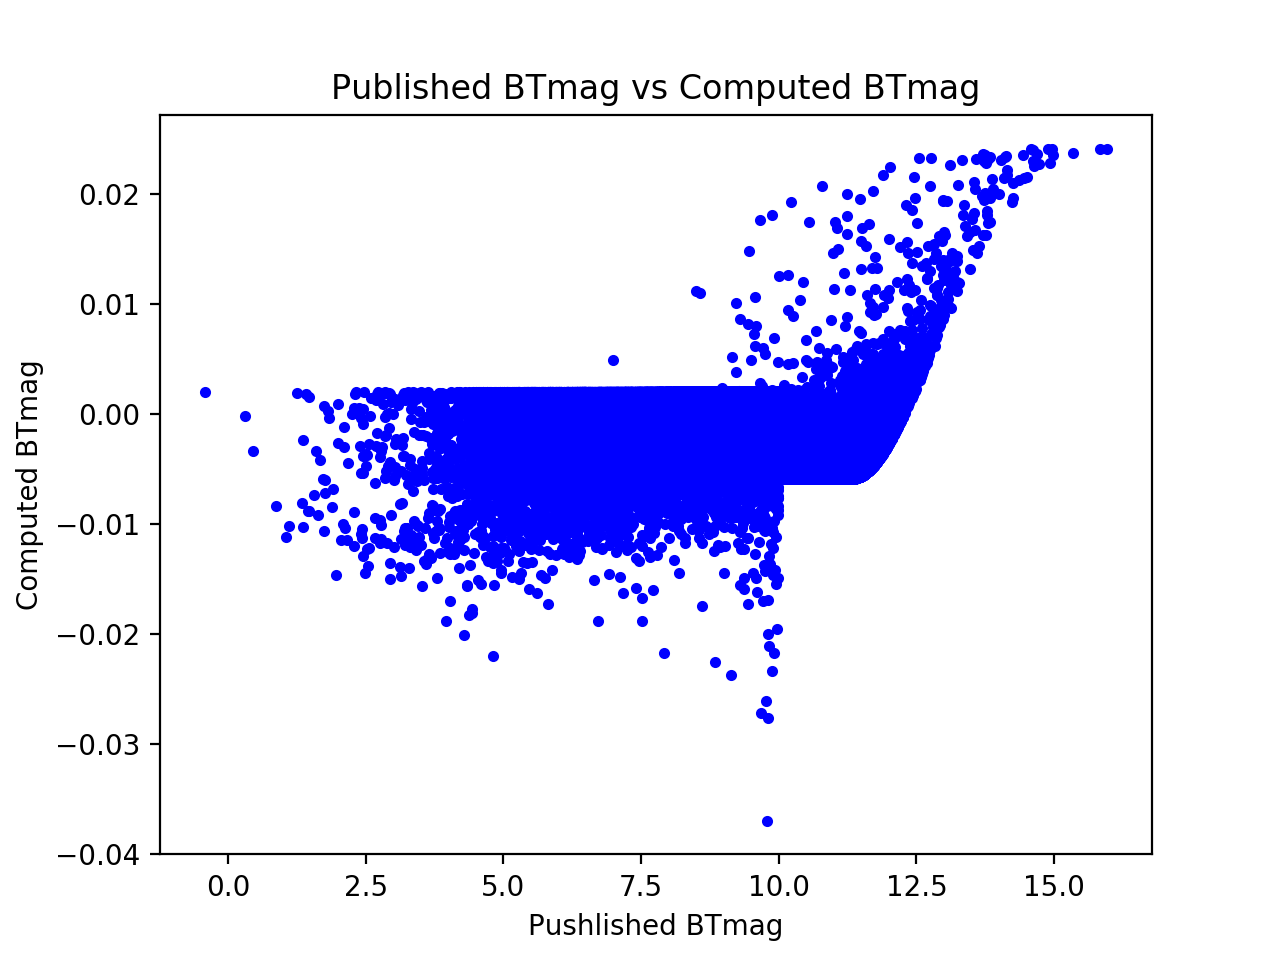
\includegraphics[height=2.3in]{btmag_error}
    \end{subfigure}%
    ~ 
    \begin{subfigure}
        \centering
        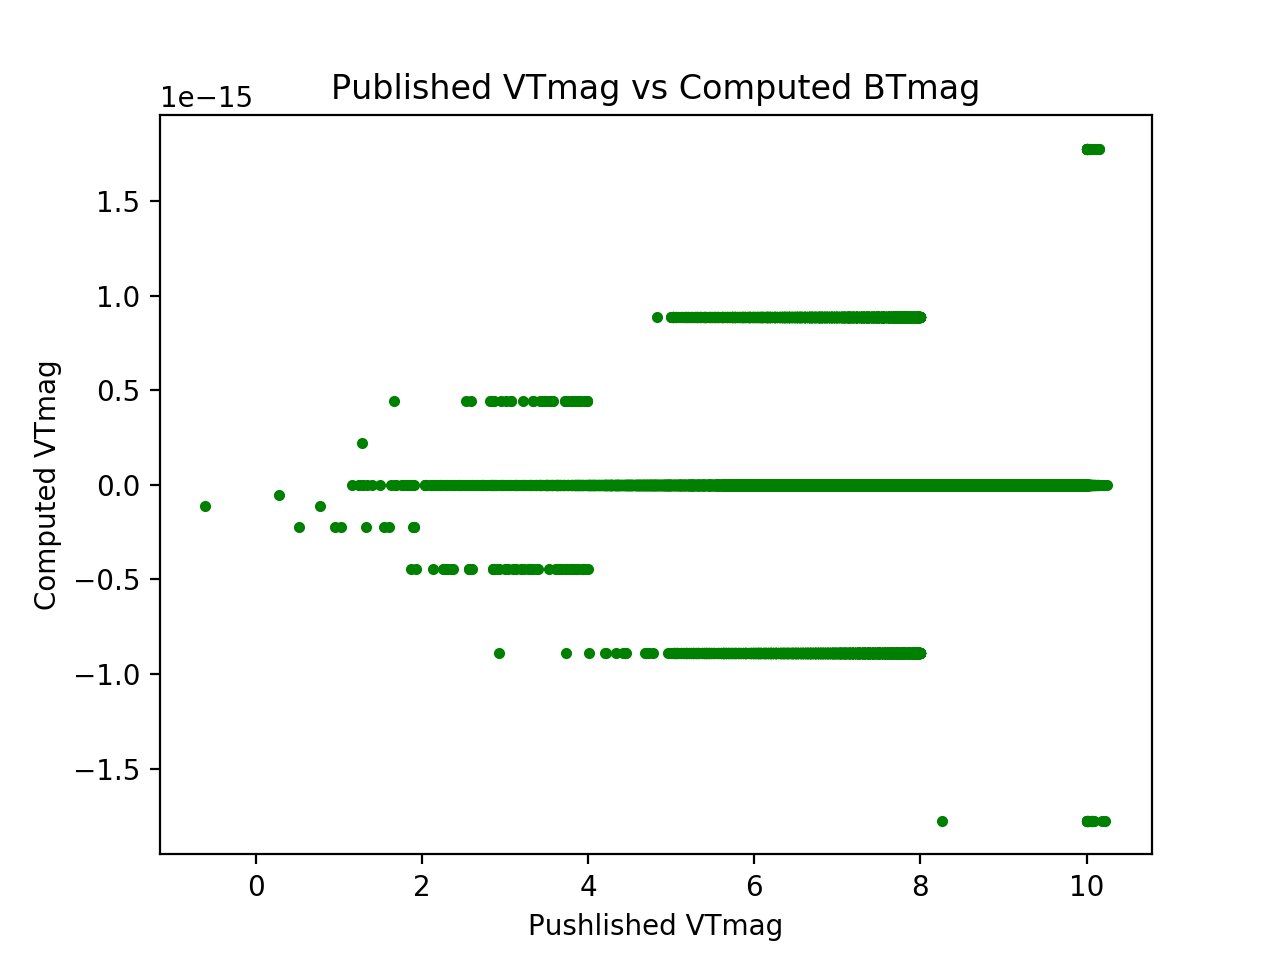
\includegraphics[height=2.3in]{vtmag_error}
    \end{subfigure}
    \caption{Magnitude Errors for Tycho Blue and Visible Filters. Note that VTmag errors are on the order of $1e-15$ and that binning is consistent with machine error.}
\end{figure*}


\begin{figure*}[t!]
    \centering
    \begin{subfigure}
        \centering
        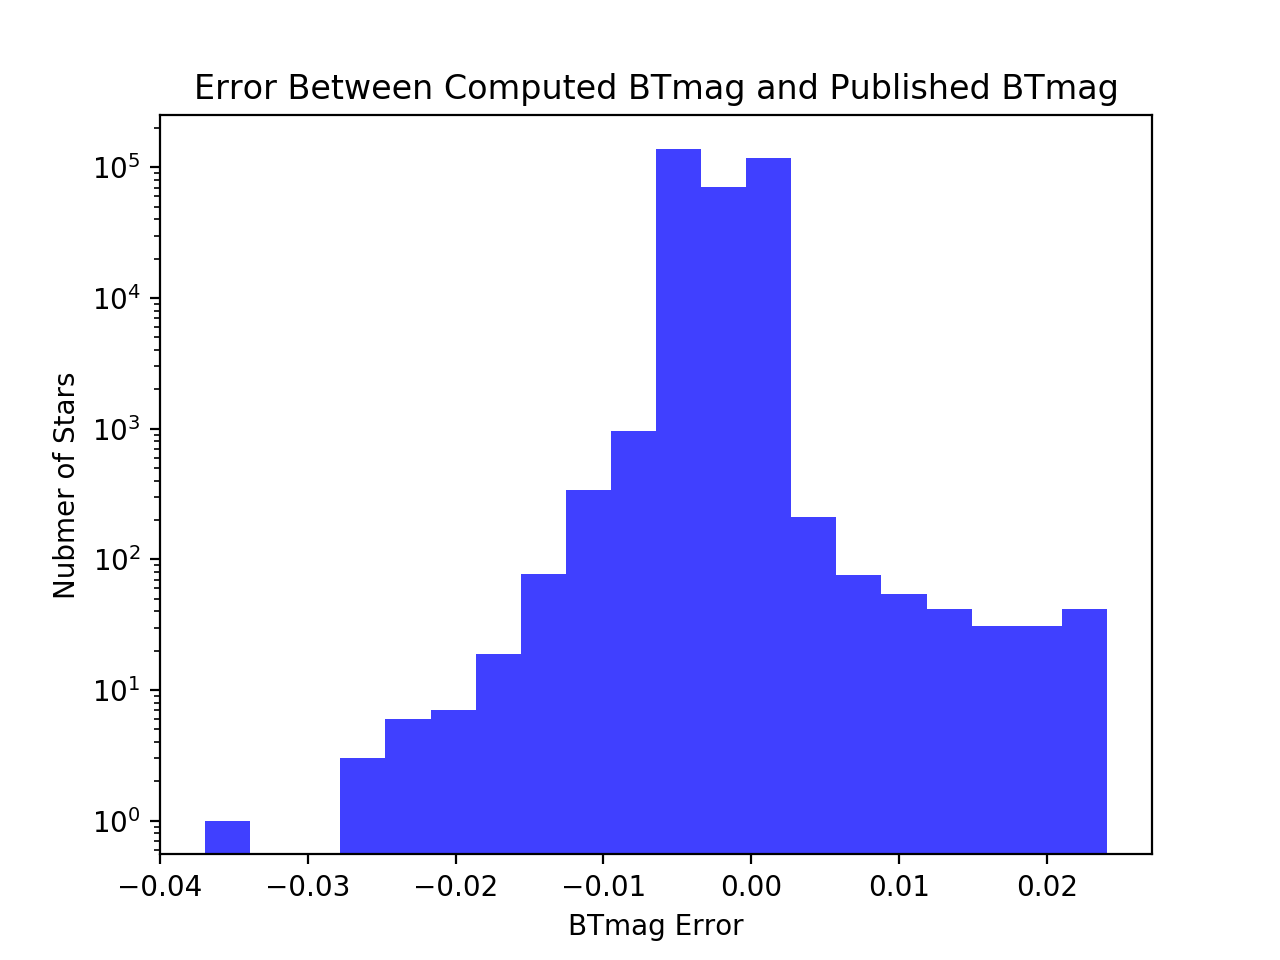
\includegraphics[height=2.3in]{btmag_hist}
    \end{subfigure}%
    ~ 
    \begin{subfigure}
        \centering
        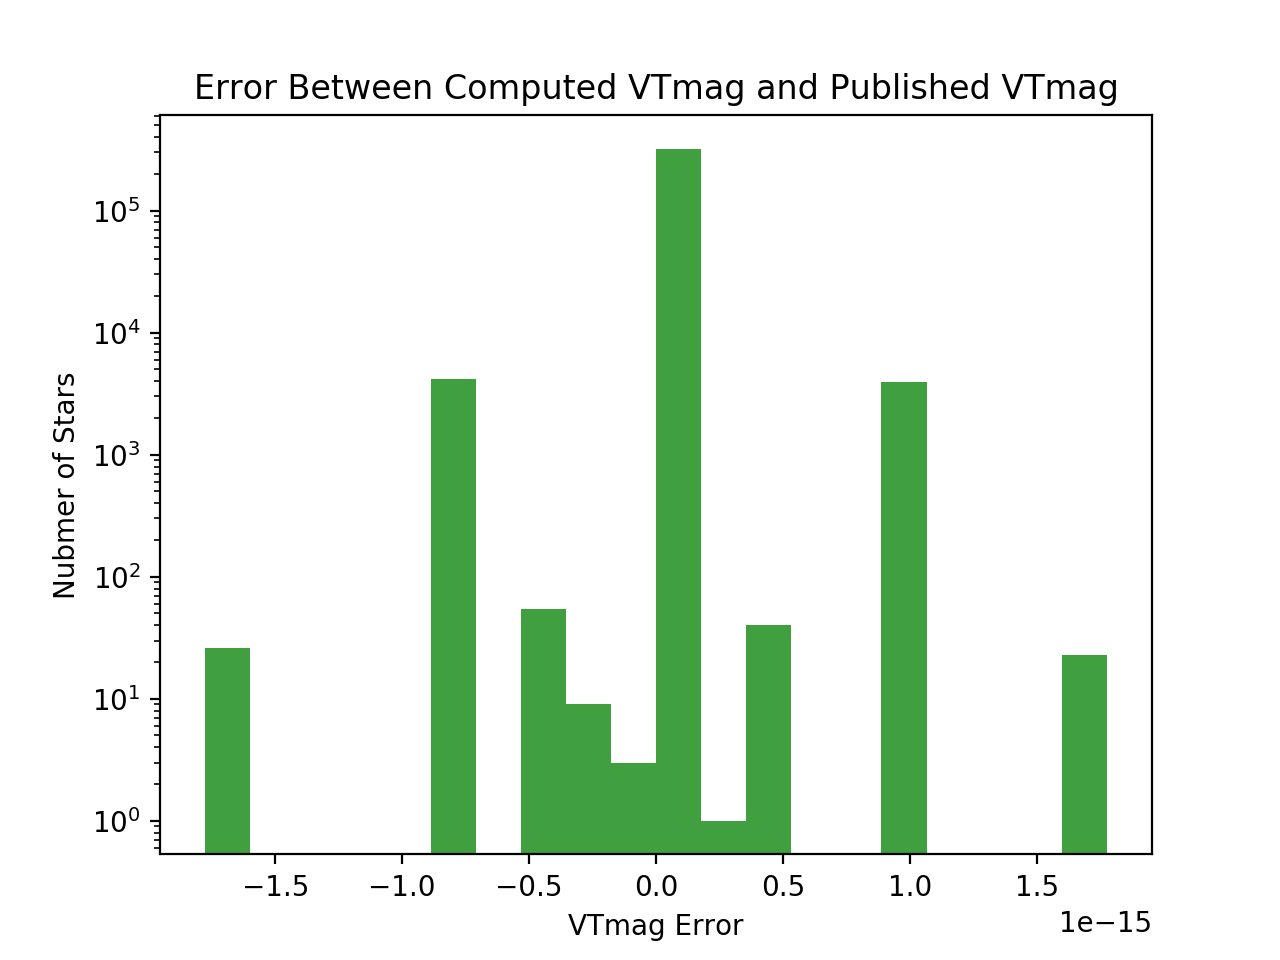
\includegraphics[height=2.3in]{vtmag_hist}
    \end{subfigure}
    \caption{Sensitivity curves for B and V filters for both Tycho and Johnson. Both are overlaid with a normalized blackbody for Vega with an effective temperature of 9550K.}
\end{figure*}


\section{Caveats} \\
\begin{enumerate}
    \item \textit{Some exotic stars are problematic.}\\
    Of all the stars presented in the scatter plots above, the clearest outlier is Gamma Velorum, with a published temperature of 57,000K and a computed temperature of 4992K. Gamma Velorum is a spectroscpoic binary, the brighter of which is a Wolf-Rayet star. Because such stars have dramatically different spectra than a true blackbody, we are not surprised that its fit is so poor. Despite the existence of such stars, we propose to continue with the assumption that all stars are well approximated by blackbodies because such outliers tend to be exceedingly rare. However, because Gamma Velorum is so bright and will clearly be detected by any camera modeled, we may want to revisit it as a special case if time permits later in the project.
    \item \textit{Not all stars have $B_T$ and $V_T$ values in the Tycho-2 database.} \\
    Of the 329,499 stars  used by DINO C-REx from the Tycho-2 database, 256 are without entries for either $B_T$ (255 stars) or $V_T$ (1 star). These include some of the brightest (like Sirius) and dimmest stars. Of these, 180 have Hipparchos IDs, meaning that other metrics (like Johnson color index or Temperature) may be available from other catalogs, and realistic approximations should be available for relatively little cost. For immediate development purposes, the DINO C-REx team proposes treating all such stars as having a color index of zero, with the hope of collecting more realistic data as time permits later in the project. However, it is likely that we will never find a better method to approximate the 76 remaining stars without a Hipparchos ID.
    \item \textit{Fig \ref{T_scatter} shows significant problem with blackbody assumption}. \\
    While the model is verified to high confidence by the computation of $B_T$, fig \ref{T_scatter} points to a central problem of the model. Where temperatures are incorrect, total fluxes will be as well. This is likely due to deviations of the spectra of real stars from the blackbody curve assumed in the model. However, because the model correctly returns reasonable values for $B_T$ and $V_T$, we feel that it is sufficient. It is likely that any filters used in an optical system will be similar enough to those used on the Tycho spacecraft, that the approximation will suffice.
\end{enumerate}
\section{Recommendations}  \\
Although the DINO C-REx camera team recommends that the method described above be implemented in its model, we have also identified some improvements that can be made. We recommend that they be implemented later in development as time permits as the Camera Model can be made fully functional even without them.
\begin{enumerate}
    \item \textit{Better modeling of stars with no recorded} $B_T$. As described above, many stars in the Tycho-2 catalog, including 16 of the brightest 100 stars in the sky have no $V_T$ magnitude recorded. Modeling them directly looking up either their temperatures or Johnson magnitudes in a catalog would allow them to be included in the model in a more realistic way than the method proposed above (setting $(B-V)_T=0$ for all). The greatest burden of this method would be in data collection rather than in computer modeling.
    \item \textit{Divergence of very hot stars from a linear fit}. \\
    Here the Camera team proposes spending some more time with lmfit, this time trying to fit a more sophisticated function to the computed/published temperature data. Figure \ref{T_scatter} above clearly shows a trend that could be better modeled with a function with a form similar to:
    \begin{equation}
        T_{published} = a + bT_{computed} - c(d + T_{computed})^f
    \end{equation}
\end{enumerate}


\end{document}
